\setcounter{section}{0}

\Needspace{5\baselineskip}
\hypertarget{ux5177ux8eabux667aux80fdux8badux7ec3ux6570ux636eux6982ux8ff0}{%
\section{具身智能训练数据概述}\label{ux5177ux8eabux667aux80fdux8badux7ec3ux6570ux636eux6982ux8ff0}}

缺乏足够的训练数据是具身智能发展的一大难题。不同数据的量和价值各有不同。

\Needspace{5\baselineskip}
\hypertarget{ux4e00ux771fux673aux6570ux636e}{%
\subsection{一、真机数据}\label{ux4e00ux771fux673aux6570ux636e}}

\Needspace{5\baselineskip}
这是精度和价值最高的一类数据，可以由人类操作员通过遥操作设备控制真实机器人完成任务产生，也可以由经过预训练的模型自主执行任务产生（失败边缘时，人类专家可介入进行修正，产生从失误中恢复的数据）。其中，遥操作的方式较多，下面举几个例子：

\begin{enumerate}
\def\labelenumi{\arabic{enumi}.}
\item
  直接输入，人通过手柄、摇杆、键盘、鼠标、触摸屏等设备直接给机器人发送运动指令，但对高自由度任务实现难度大。
\item
  主从式，操作者控制一个``主设备''，机器人作为``从设备''同步运动，如远端机械臂跟随主机械臂的位置和姿态。
\item
  动捕，把人的动作重定向到机器人，与人的日常动作相对契合度高，但笨重的设备下人的动作容易变形、产出高质量数据效率也不够高，且部分动作机器人难以复现。
\item
  利用VR/AR设备等，操作者戴 VR 头显，在虚拟或增强现实环境中观察机器人视角，并通过手柄、手部追踪等方式控制机器人。
\end{enumerate}

优点：包含了真实世界中极其复杂的物理交互，如摩擦力、形变、复杂的接触力学以及真实的光影变化，不存在``Sim-to-Real''鸿沟。

\Needspace{5\baselineskip}
缺点：

\begin{enumerate}
\def\labelenumi{\arabic{enumi}.}
\item
  采集成本极高，难以规模化。
\item
  依赖封闭的空间，任务和环境的多样性受限。
\end{enumerate}

\Needspace{5\baselineskip}
\hypertarget{ux4e8cux7269ux7406ux5f15ux64ceux5408ux6210ux6570ux636e}{%
\subsection{二、物理引擎合成数据}\label{ux4e8cux7269ux7406ux5f15ux64ceux5408ux6210ux6570ux636e}}

可利用物理仿真引擎在虚拟世界中构建环境，通过强化学习或大规模并发采样获取数据。

\Needspace{5\baselineskip}
优点：

\begin{enumerate}
\def\labelenumi{\arabic{enumi}.}
\item
  可以快速收集海量试错数据、轻易获取环境的真实状态（如物体的精确位姿、接触力）。
\item
  环境比真机数据更加多样。
\end{enumerate}

缺点：存在Sim-to-Real Gap，物理引擎无法完美模拟现实世界，特别是对于流体、柔性物体、复杂的滑动摩擦、触觉传感器，以及各种意外情况的模拟等。

\Needspace{5\baselineskip}
\hypertarget{ux4e09ux4e92ux8054ux7f51ux89c6ux9891ux6570ux636e}{%
\subsection{三、互联网视频数据}\label{ux4e09ux4e92ux8054ux7f51ux89c6ux9891ux6570ux636e}}

互联网中存在海量的视频数据，其中蕴含了丰富的常识、物理规律以及``如何与世界交互''的知识，可用于具身模型的预训练等，帮助模型理解物理世界的基本规律。

优点：数据量大，多样性高，可增强模型跨场景的泛化能力。

\Needspace{5\baselineskip}
缺点：

\begin{enumerate}
\def\labelenumi{\arabic{enumi}.}
\item
  人类的身体构造（自由度、肌肉骨骼系统）与机器人完全不同，存在Embodiment Gap。一段人类灵活切菜的视频，很难直接转化为带有两指夹爪的机械臂的电机控制指令。
\item
  只有像素变化，缺乏动作标签。
\end{enumerate}

\Needspace{5\baselineskip}
\hypertarget{ux56dbumiux53caux53efux7a7fux6234ux8bbeux5907ux91c7ux96c6ux6570ux636e}{%
\subsection{四、UMI及可穿戴设备采集数据}\label{ux56dbumiux53caux53efux7a7fux6234ux8bbeux5907ux91c7ux96c6ux6570ux636e}}

UMI（Universal Manipulation Interface）是一类面向机器人操作的数据采集方案。采集员通常手持带有相机、位姿传感器和夹爪等组件的便携式设备，在真实环境中直接完成抓取、整理、开关门等操作，并记录第一视角视觉、末端执行器位姿、夹爪开合状态等信息，之后再将人类操作轨迹映射到机器人上。此外，还有通过可穿戴外骨骼采集数据的方案，同样可以在真实环境中采集数据，并在后续将相关轨迹映射到机器人上。

\Needspace{5\baselineskip}
优点：

\begin{enumerate}
\def\labelenumi{\arabic{enumi}.}
\item
  数据直接来源于真实世界，又比真机遥操作更轻便、成本更低，不受机器人本体数量限制。
\item
  采集员可以直接利用人类灵活的运动能力完成复杂任务。
\end{enumerate}

缺点：采集设备与实际机器人仍存在一定的Embodiment Gap，主要记录末端执行器的运动轨迹，无法完整复现机器人执行过程中的一些信息。

\Needspace{5\baselineskip}
\hypertarget{ux4e94ux4ebaux7c7bux7b2cux4e00ux89c6ux89d2ux89c6ux9891ux6570ux636e}{%
\subsection{五、人类第一视角视频数据}\label{ux4e94ux4ebaux7c7bux7b2cux4e00ux89c6ux89d2ux89c6ux9891ux6570ux636e}}

通过头戴式相机、智能眼镜或胸前相机等设备，记录人类在真实生活环境中完成做饭、整理、维修、装配等任务时的第一视角视频。

\Needspace{5\baselineskip}
优点：

\begin{enumerate}
\def\labelenumi{\arabic{enumi}.}
\item
  成本低，规模化潜力强。
\item
  与普通互联网视频相比，这类数据的视角更加接近机器人执行任务时的观察视角，并且包含大量连续的人---物交互过程。
\end{enumerate}

\Needspace{5\baselineskip}
缺点：

\begin{enumerate}
\def\labelenumi{\arabic{enumi}.}
\item
  以视频像素为主，缺少机器人的动作标签，且人手与机器人存在明显的Embodiment Gap。
\item
  存在严重的手部和物体遮挡、快速相机运动以及视角抖动等，使得三维轨迹恢复和动作识别较为困难。
\end{enumerate}

\Needspace{5\baselineskip}
\hypertarget{ux516dux4e16ux754cux6a21ux578bux751fux6210ux6570ux636e}{%
\subsection{六、世界模型生成数据}\label{ux516dux4e16ux754cux6a21ux578bux751fux6210ux6570ux636e}}

世界模型通过学习真实世界或机器人交互数据中的状态转移规律，预测在给定当前状态和动作的情况下未来环境会如何变化。让智能体在世界模型中进行大量Rollout，可获取大量数据。

\Needspace{5\baselineskip}
优点：

\begin{enumerate}
\def\labelenumi{\arabic{enumi}.}
\item
  成本低，获取速度快。
\item
  可覆盖真实数据中数量较少的corner case和模拟极端环境等。
\end{enumerate}

\Needspace{5\baselineskip}
缺点：

\begin{enumerate}
\def\labelenumi{\arabic{enumi}.}
\item
  误差可能会累积，当前不能保证符合物理世界的真实规律。
\item
  目前对于精细接触、摩擦、形变、力觉和触觉等建模能力还有限。
\end{enumerate}

\Needspace{5\baselineskip}
\hypertarget{ux4e03ux6570ux636eux7ec4ux5408ux914dux65b9}{%
\subsection{七、数据组合配方}\label{ux4e03ux6570ux636eux7ec4ux5408ux914dux65b9}}

\Needspace{5\baselineskip}
在具身智能模型的训练中，往往会根据不同类型数据的特点，组合运用各类数据，优化数据配方。以GigaWorld-Policy的训练过程为例：

\begin{enumerate}
\def\labelenumi{\arabic{enumi}.}
\item
  通用物理世界预训练：先利用海量互联网视频数据进行预训练，让模型建立起对通用物理规律和视觉动态的基础认知。
\item
  具身场景后训练：利用涵盖第一人称、真机及仿真的多源操作视频进行后训练。在这一阶段，掌握具身交互场景下的时空演变规律和基本操作方法。
\item
  小样本的动作对齐：只需少量的真机动作标签数据进行训练，即可将预训练世界模型与机器人的动作预测对齐，快速打通``观测-动作-未来视觉''的因果映射。
\end{enumerate}

\begin{figure}[htbp]
\centering
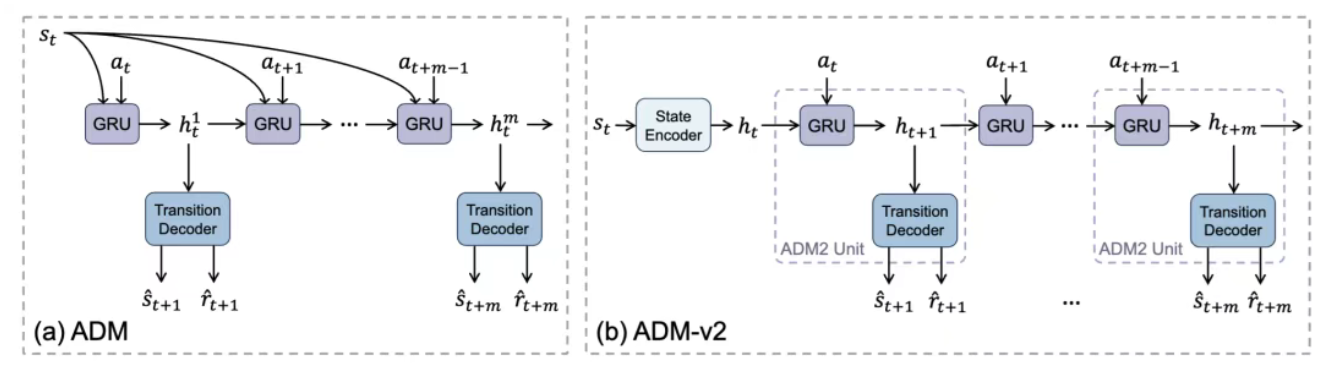
\includegraphics{images/image-0052.png}
\caption{GigaWorld-Policy 的训练与推理数据配方}
\end{figure}

\FloatBarrier
\Needspace{5\baselineskip}
\hypertarget{ux53c2ux8003ux6587ux732e-162}{%
\subsection{参考文献}\label{ux53c2ux8003ux6587ux732e-162}}

\vspace{0.25em}
\begin{itemize}
\tightlist
\item
  Open X-Embodiment Collaboration. (2023). \href{https://arxiv.org/abs/2310.08864}{Open X-Embodiment: Robotic Learning Datasets and RT-X Models}. arXiv:2310.08864.
\item
  Khazatsky, A., Pertsch, K., Nair, S., et al.~(2024). \href{https://arxiv.org/abs/2403.12945}{DROID: A Large-Scale In-The-Wild Robot Manipulation Dataset}. arXiv:2403.12945.
\item
  Chi, C., Xu, Z., Pan, C., et al.~(2024). \href{https://arxiv.org/abs/2402.10329}{Universal Manipulation Interface: In-The-Wild Robot Teaching Without In-The-Wild Robots}. arXiv:2402.10329.
\item
  Xu, M., Zhang, H., Hou, Y., et al.~(2025). \href{https://arxiv.org/abs/2505.21864}{DexUMI: Using Human Hand as the Universal Manipulation Interface for Dexterous Manipulation}. arXiv:2505.21864.
\item
  X Square Robot. (2026). \href{https://x2robot.com/en/pages/twindex}{TwinDEX --- Dexterous. Consistent. Scalable}. Project page.
\item
  Zheng, R., Niu, D., Xie, Y., et al.~(2026). \href{https://arxiv.org/abs/2602.16710}{EgoScale: Scaling Dexterous Manipulation with Diverse Egocentric Human Data}. arXiv:2602.16710.
\item
  Ye, A., Wang, B., Ni, C., et al.~(2026). \href{https://arxiv.org/abs/2603.17240}{GigaWorld-Policy: An Efficient Action-Centered World-Action Model}. arXiv:2603.17240.
\end{itemize}

\clearpage
